%Auhor Honorio Apaza (honorio.apz@gmail.com)
%Para hacer informe con portada utilizamos report

\documentclass[12pt]{report}

\usepackage[a4paper]{geometry}
\usepackage[myheadings]{fullpage}
\usepackage{fancyhdr}
\usepackage{lastpage}
\usepackage{graphicx, wrapfig, subcaption, setspace, booktabs}
\usepackage[T1]{fontenc}
\usepackage[font=small, labelfont=bf]{caption}
\usepackage{fourier}
\usepackage[protrusion=true, expansion=true]{microtype}
\usepackage{setspace}

%Paquete para hipervinculos
\usepackage[colorlinks=true]{hyperref}
\hypersetup{
    colorlinks=true,
    linkcolor=black,
    filecolor=magenta,      
    urlcolor=blue,
    citecolor=black,
}

%Para qué los subtítulos aparezcan en español
\usepackage[spanish]{babel}
\usepackage[utf8]{inputenc}
\usepackage{sectsty}
\usepackage{url, lipsum}
\usepackage{tabularx}
\usepackage{float}

%--------------------------------------------------
%Para agregar citas en apaKdTree-Knn
%Para citar se usa el comando \cite{}
%Las referencias se modifican en el archivo sample.bib
\usepackage{apacite}
%----------------------------------------------

\newcommand{\HRule}[1]{\rule{\linewidth}{#1}}
\onehalfspacing
\setcounter{tocdepth}{5}
\setcounter{secnumdepth}{5}

%-------------------------------------------------------------------------------
%Encabezado y pie de pagina y numeracion
%\fancyhead para encabezado
%\fancyfoot para pie de pagina
% L para izquierda, left
% R para derecha, right
% C para centro, center
%-------------------------------------------------------------------------------
\pagestyle{fancy}
\fancyhf{}
\setlength\headheight{15pt}
\fancyhead[L]{\chaptername \ \thechapter} 
\fancyhead[R]{Universidad Nacional de Moquegua}
\fancyfoot[R]{\thepage}

\begin{document}
%-------------------------------------------------------------------------------
% Portada
%-------------------------------------------------------------------------------
\begin{titlepage}
\centering
{\bfseries\LARGE UNIVERSIDAD NACIONAL DE MOQUEGUA \par}
\vspace{0.2cm}
{\scshape\LARGE Ingeniería de Sistemas e Informática \par}
\vspace{1cm}
{
\includegraphics[width=0.3\textwidth]{Logo_EPISI.png}\par}
\vspace{1cm}
%\vspace{3cm}
{\Large Proyecto de investigación:  \par}
\vspace{1cm}

{\bfseries\scshape\LARGE Titulo de proyecto de investigación para la obtención del titulo profesional \par}
\vspace{1cm}
{\Large Presentado por: \par}
{\Large Nombre del autor  \par}
\vfill
{\Large Asesor: \par}
{\Large Nombres del asesor \par}
\vfill
{\bfseries\Large Ilo, Agosto del 2021 \par}
\end{titlepage}




%se debe incluir el comando \maketitle para hacer 
%\maketitle

%Para hacer el índice solo es necesario agregar 
\tableofcontents
\listoffigures
\listoftables
\newpage

%-------------------------------------------------------------------------------
% Section title formatting
%\sectionfont{\scshape}
%-------------------------------------------------------------------------------

%-------------------------------------------------------------------------------
% BODY
%-------------------------------------------------------------------------------

\chapter{Introducción}
 


\section{Descripción y formulación del problema}
Primera cita"  \cite{2020arXiv200711053A}, Segunda cita \cite{2021arXiv210401765A}.


\section{Antecedentes}
Aquí se escribe justificación..
\section{Objetivos}
\subsection{Objetivo general}
Aquí van los Objetivos...
\subsection{Objetivos específicos}
\begin{itemize}
\item Objetivo 1
\item Objetivo 2
\end{itemize}

\section{Justificación e importancia}
Aquí va justificación...

\section{Hipótesis (opcional)} 
\begin{itemize}
\item Hipótesis 1
\item Hipótesis 2
\end{itemize}

\chapter{Marco teórico}
\section{Bases teóricas}

... Ejemplo de referencia a Figura \ref{Figura_diferencias_AI_DS_ML}.
\begin{figure}[H]
\centering
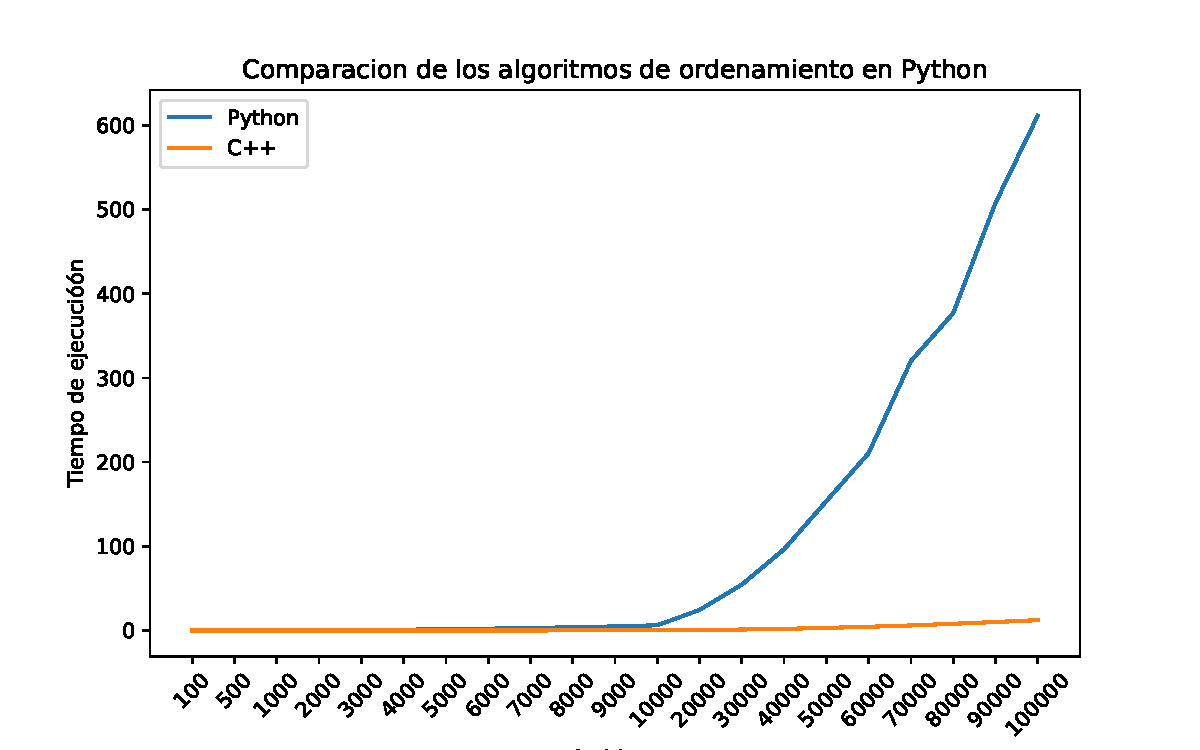
\includegraphics[width=6in]{countingSort.pdf}
\caption{Comparación del tiempo de ejecución entre Python y C++.}%\cite{wikepedia}
\label{Figura_diferencias_AI_DS_ML}
\end{figure}

\section{Definición de términos}
\begin{itemize}
    \item Termino 1\\
    \item Termino 2\\
\end{itemize}

\chapter{Metodologías}
\section{Procedimientos}


\section{Análisis de datos}

\chapter{Aspectos administrativos}

\section{Cronograma de actividades}
Texto aquí... 
\begin{table}[htpb]
\centering
\caption{Cronograma de actividades de proyectos.}
\begin{tabular}{ccccc}
\toprule
Actividades & \multicolumn{4}{c}{Meses} \\
&Agosto & Setiembre & Octubre & Noviembre \\
\midrule
Nombre de actividad & X & &  &  \\
Nombre de actividad & & X &  &  \\
Nombre de actividad & & X &  &  \\
Nombre de actividad & & X &  &  \\
Nombre de actividad &  & & X &  \\
Nombre de actividad &  & & X &  \\
Nombre de actividad &  & &  & X \\
\bottomrule
\end{tabular}

\bigskip
\small\textit{Nota}. Una nota por aquí.
\end{table}

\section{Presupuesto}
 En la tabla \ref{table_presu} se detalla el presupuesto necesario para la ejecución del proyecto...
\begin{table}[H]
\centering
\caption{Presupuesto de proyecto.}
\begin{tabular}{ccc}
\toprule
Actividades & \multicolumn{2}{c}{Presupuesto} \\
&Materiales & Presupuesto  \\
\midrule
Nombre de actividad & Laptop & s/. 2000.00 \\
Nombre de actividad & Laptop, internet, luz eléctrica & S/. 100.00  \\
Nombre de actividad &Laptop, internet, luz eléctrica & S/. 100.00  \\
Nombre de actividad & Laptop, internet, luz eléctrica& S/. 100.00   \\
Nombre de actividad & Laptop, internet, luz eléctrica & S/. 100.00  \\
Nombre de actividad & Laptop, internet, luz eléctrica & S/. 100.00 \\
Nombre de actividad & Laptop, proyector &  S/. 100.00\\
TOTAL &  & S/. 2600.00 \\
\bottomrule
\end{tabular}
\bigskip
%\small\textit{Nota}. Los gatos y material necesario adicional sera asumido por el autor .
\label{table_presu}
\end{table}
 
\section{Fuente de financiamiento}
Texto aquí.


%--------------------------------TABLAS-------------
%Insertar tabla
% Las tablas se pueden generar a través de:
% www.tablegenerator.com
%---------------------------------------------------




%-------------------------------------------------------------------------------
% REFERENCIAS
%-------------------------------------------------------------------------------
\newpage

\bibliographystyle{apacite}
\bibliography{sample.bib}



\end{document}

%-------------------------------------------------------------------------------
% SNIPPETS
%-------------------------------------------------------------------------------

%\begin{figure}[!ht]
%	\centering
%	\includegraphics[width=0.8\textwidth]{file_name}
%	\caption{}
%	\centering
%	\label{label:file_name}
%\end{figure}

%\begin{figure}[!ht]
%	\centering
%	\includegraphics[width=0.8\textwidth]{graph}
%	\caption{Blood pressure ranges and associated level of hypertension (American Heart Association, 2013).}
%	\centering
%	\label{label:graph}
%\end{figure}

%\begin{wrapfigure}{r}{0.30\textwidth}
%	\vspace{-40pt}
%	\begin{center}
%		\includegraphics[width=0.29\textwidth]{file_name}
%	\end{center}
%	\vspace{-20pt}
%	\caption{}
%	\label{label:file_name}
%\end{wrapfigure}

%\begin{wrapfigure}{r}{0.45\textwidth}
%	\begin{center}
%		\includegraphics[width=0.29\textwidth]{manometer}
%	\end{center}
%	\caption{Aneroid sphygmomanometer with stethoscope (Medicalexpo, 2012).}
%	\label{label:manometer}
%\end{wrapfigure}

